\chapter{Android 5 – Intents, App-Widgets, Fragments \& Support Library}

\section{Intents: Filter \& Auflösung}

In Android gibt es explizite Intents oder implizite Intents. Explizite Intents werden über den Fully-Qualified-Classname der Ziel-Komponenten aufgerufen und wird typischerweise für App-interne Zwecke verwendet. Implizite Intents erlauben eine späte Bindung zur Laufzeit zwischen Code in verschiedenen Apps. Der Intent ist eine passive Datenstruktur (er macht nichts), welche eine abstrakte Beschreibung einer Aktion enthält. Das System kümmert sich um die Auslieferung des Intents an die richtige Komponente.
Da bei impliziten Intents der Empfänger nicht von vornherein feststeht, muss der Intent mittels eines Intent-Filters ausgewählt werden. Das System eruiert mögliche Empfänger (Intent Auflösung), dabei kann es zu drei möglichen Fällen kommen:
\begin{enumerate}
	\item Ein Empfänger wurde gefunden $\leftarrow$ direkte Zustellung
	\item Mehrere Empfänger wurden gefunden $\leftarrow$ Benutzer wählt mit Dialog aus
	\item Kein Empfänger gefunden $\leftarrow$ \texttt{ActivityNotFoundException}
\end{enumerate}
Ein impliziter Intent enthält folgende Informationen:
\begin{description}
	\item[Action:] Der Typ der Aktion, die ausgeführt werden soll, z.B. ACTION\_VIEW, ACTION\_EDIT, MY\_CUSTOM\_ACTION usw.
	\item[Category:] Kategorie der Komponenten, welche diesen Intent ausführen soll, z.B. DEFAULT, LAUNCHER, BROWSABLE (eine Komponente welche sicher von einem Browser aufgerufen werden kann)
	\item[Data:] Die Daten, mit welchen gearbeitet werden soll (URI und Mime Type)
	\item[Extras:] Schüssel/Wert-Paare für Zusatzinformationen
\end{description}
Die oben genannten Informationen werden auch bei einem Intent-Filter im Manifest definiert. Ein Intent-Filter kann einer Activity oder einem Service zugeordnet werden. Das System vergleicht nun den Action, die Category und das Data mit den Intent-Filtern und an dessen Intent-Filter wo alles übereinstimmt, wird der Intent zur Verarbeitung übergeben. Abbildung \ref{fig:impliziter-intent} zeigt wie ein impliziter Intent mit Action und Data erzeugt wird. Das Bild in der Mitte erklärt wie der entsprechende Intent-Filter im Manifest deklariert wird. Das letzte Bild zeigt wie die Daten eines Intents in der dazugehörigen Activity ausgelesen werden.
\begin{figure}
	\centering
	\begin{subfigure}[b]{0.3\textwidth}
		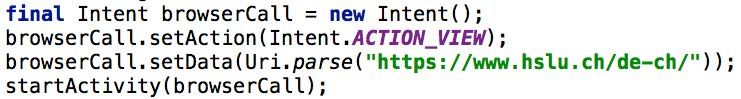
\includegraphics[width=\textwidth]{fig/impliziter-intent-aufruf}
		\caption{Aufruf eines impliziten Intents}
	\end{subfigure}
	~
	\begin{subfigure}[b]{0.3\textwidth}
		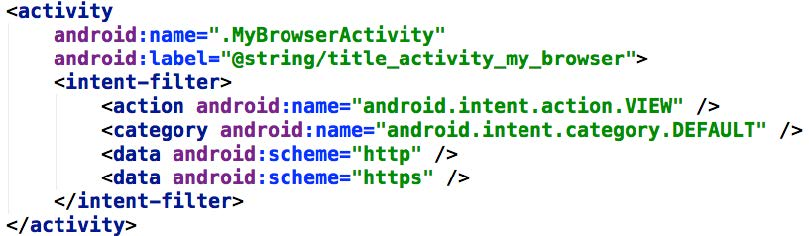
\includegraphics[width=\textwidth]{fig/impliziter-intent-xml}
		\caption{Deklaration Intent-Filter}
	\end{subfigure}
	~
	\begin{subfigure}[b]{0.3\textwidth}
		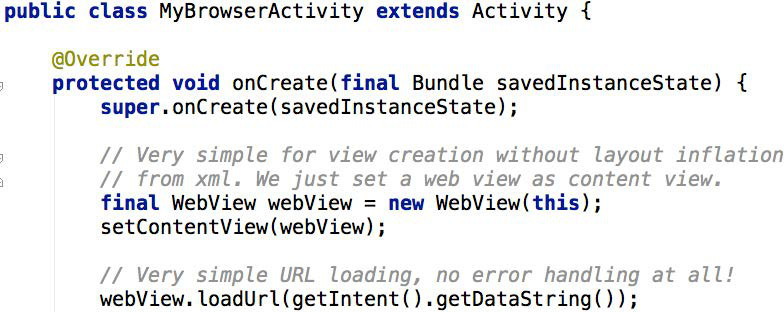
\includegraphics[width=\textwidth]{fig/impliziter-intent-activity}
		\caption{Daten vom Intent auslesen}
	\end{subfigure}
	\caption{Impliziter Intent}
	\label{fig:impliziter-intent}
\end{figure}
Mit der Klasse \texttt{PackageManager} kann die  Intent-Auflösung abgefragt werden. Die Methoden die mit \texttt{query\dots()} beginnen liefern alles passenden Intents (z.B. alle die Browser-Intents verstehen) zurück. Die Methoden die mit \texttt{resolve\dots()} beginnen liefert den best-passenden Intent zurück.

\section{Fragments}

Fragments sind eine Art \emph{Sub-Activity}, welche in verschiedenen Activities wiederverwendet werden kann. Sie wurden mit Android 3 eingeführt und haben das Ziel Tablett-Unterstützung zu ermöglichen. Fragments haben einen eigenen Lebenszyklus, eigene Input-Events und können zu einer laufenden Activity hinzugefügt oder entfernt werden. Abbildung \ref{fig:fragment-design} sollte das Prinzip nochmal verdeutlichen.

\begin{figure}
\centering
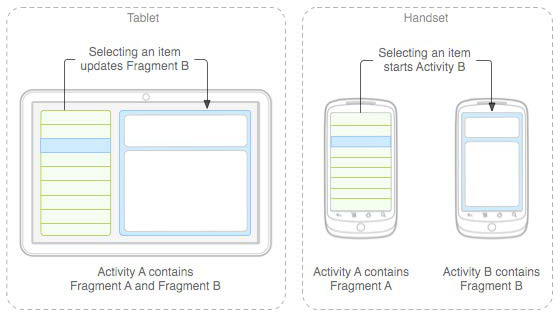
\includegraphics[width=0.7\linewidth]{fig/fragment-design}
\caption{Fragement Design-Philosophie}
\label{fig:fragment-design}
\end{figure}

Der Lebenszyklus von Fragments ist ähnlich wie der von Activities. Fragments können deklariert werden (layout.xml) oder programmatisch erzeugt werden. Der FragmentManager (\texttt{getFragementManager()}) verwaltet die Fragments innerhalb einer Activity. Abbildung \ref{fig:fragement-aufblasen} zeigt wie ein Fragment mit dem \texttt{LayoutInflater} erzeugt wird.

\begin{figure}
\centering
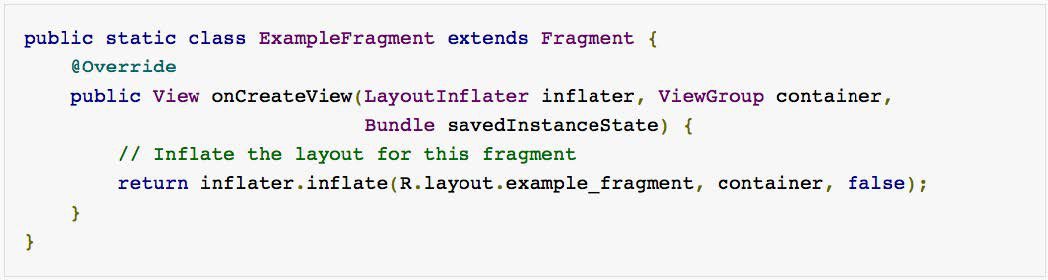
\includegraphics[width=0.7\linewidth]{fig/fragement-aufblasen}
\caption{Fragments aufblasen}
\label{fig:fragement-aufblasen}
\end{figure}

Fragments können dynamisch per Code oder deklarativ per XML zu einer Activity hinzugefügt werden.

\begin{figure}
	\centering
	\begin{subfigure}[b]{0.3\textwidth}
		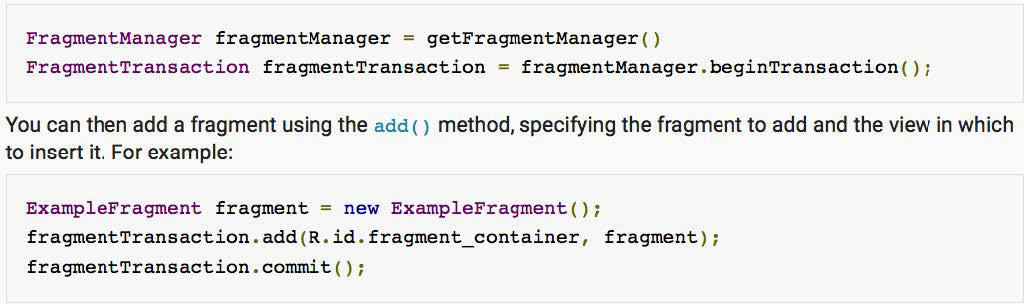
\includegraphics[width=\textwidth]{fig/fragement-activity-code}
		\caption{\texttt{FragementManager}}
	\end{subfigure}
	~
	\begin{subfigure}[b]{0.3\textwidth}
		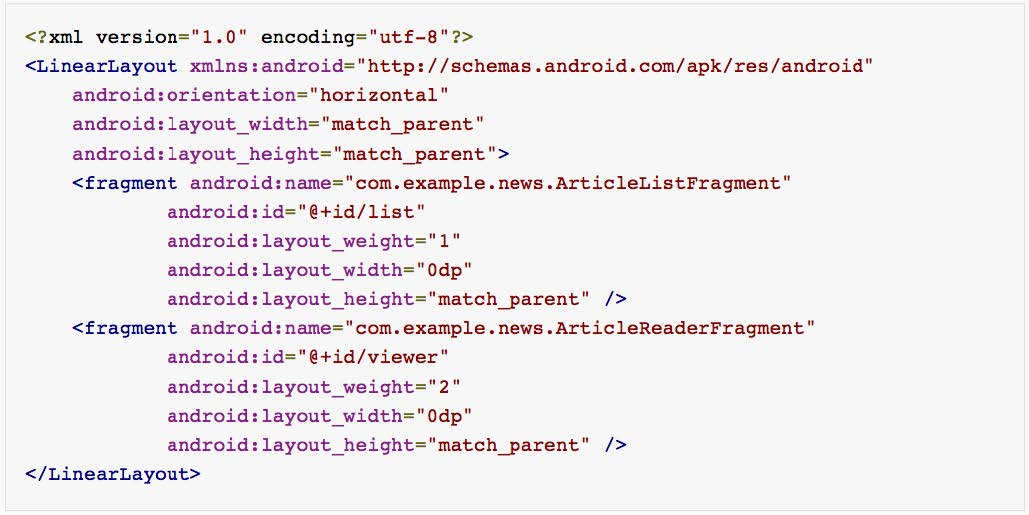
\includegraphics[width=\textwidth]{fig/fragement-activity-xml}
		\caption{XML}
	\end{subfigure}
	\caption{Fragment einer Activity hinzufügen}
	\label{fig:fragement-activity}
\end{figure}

Bei einer Activity verwaltet das System den Back-Stack (Was passiert wenn ich \emph{back} drücke?). Bei einem Fragment wird der Back Stack von der Activity verwaltet (\texttt{addToBackStack()}).

\section{App-Widgets}

Widgets sind eine Art \emph{Mini-App}, welche direkt auf dem Home-Screen sichtbar ist. Es gibt folgende Typen:
\begin{description}
	\item[Information Widgets:] Zeigen Informationen an z.B. Wetter-Widget
	\item[Collection Widgets:] Zeigt eine Sammlung von Informationen an z.B. Mail-Widget
	\item[Control Widgets:] Stellt Icons zur Verfügung z.B. um das WLAN auszuschalten
	\item[Hybrid Widgets:] Ein Kombination der obigen z.B. Musik-Widget
\end{description}
Um ein Widget zu erstellen müssen folgende Schritte durchgeführt werden:
\begin{enumerate}
	\item Widget als Receiver im Manifest deklarieren
	\item \texttt{my\_app\_widget\_provider\_info.xml} erstellen, welche Meta-Informationen zum Widget enthält (Grösse, Aktualisierungsintervall usw.)
	\item \texttt{my\_app\_widget\_provider.xml} erstellen, welche das Layout des Widgets definiert
	\item Eine \texttt{AppWidgetProvider}-Klasse erstellen, welche von \texttt{AppWidgetProvider} abgeleitet ist und die Widget-Aktualisierung vornimmt.
\end{enumerate}
Abbildung \ref{fig:widget} zeigt diese Schritte nochmals im Detail.

\begin{figure}
	\centering
	\begin{subfigure}[b]{0.4\textwidth}
		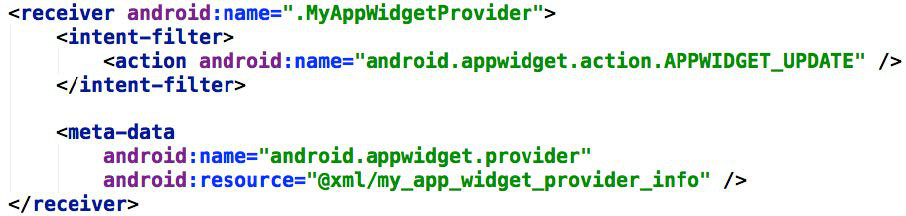
\includegraphics[width=\textwidth]{fig/widget-manifest}
		\caption{Widget im Manifest eintragen}
	\end{subfigure}
	~
	\begin{subfigure}[b]{0.4\textwidth}
		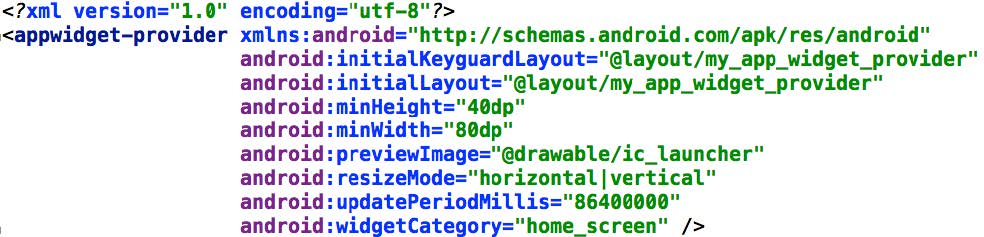
\includegraphics[width=\textwidth]{fig/widget-info}
		\caption{Metadaten deklarieren}
	\end{subfigure}
	\begin{subfigure}[b]{0.4\textwidth}
		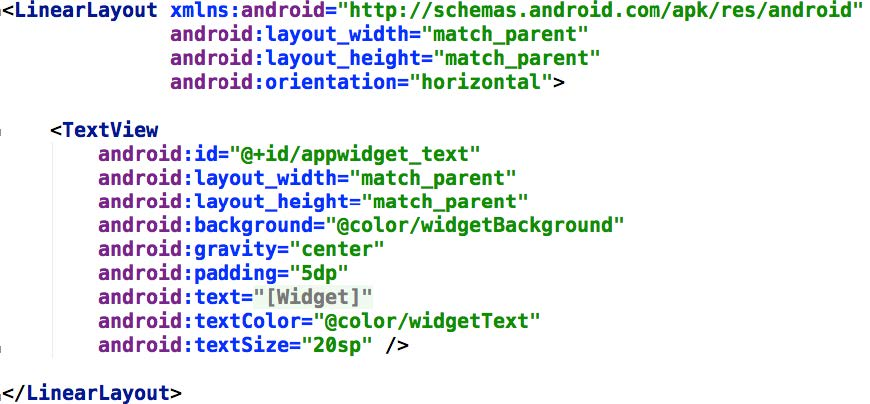
\includegraphics[width=\textwidth]{fig/widget-layout}
		\caption{Layout definieren}
	\end{subfigure}
	~
	\begin{subfigure}[b]{0.4\textwidth}
		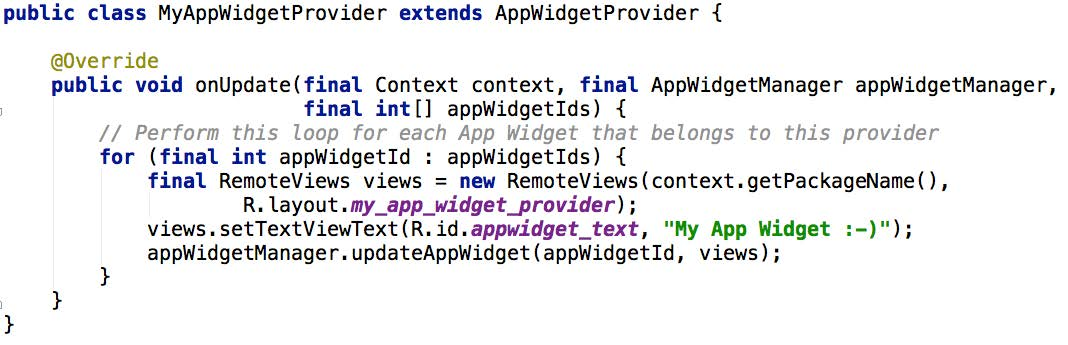
\includegraphics[width=\textwidth]{fig/widget-klasse}
		\caption{Aktualisierung}
	\end{subfigure}
	\caption{Ein Widget erstellen}
	\label{fig:widget}
\end{figure}

\section{Support Library}

Zurzeit sind immer noch sehr viel alte Android-Versionen im Einsatz (z.B. Android 2: 8\%). Damit Programmierer die neuen Möglichkeiten der API Levels nutzen können werden Support Libraries angeboten welche (ausgewählte) Funktionen für alte OS-Versionen zur Verfügung stellt. Die ActionBar gibt es z.B. erst ab Android 3.0 (nicht verfügbar auf 8\% der Geräte). Dank einer Support Library ist die ActionBar aber bis Android 2.1 verfügbar (richtige Klasse importieren).